\subsection{Bridges and infinitesimal dynamics}
\label{subsec:diffusion-bridges-dynamics}

Let \(p_0\) be the law we want to sample and let \(p_1\) be a law from which sampling is easy.
The problem is to start from \(X_1\sim p_1\) and construct a reverse-time dynamics that ends at \(p_0\).
The abstract setup has two ingredients.
First choose a joint law for the endpoint pair \((X_0,X_1)\) with marginals \(p_0\) and \(p_1\).
Then choose a bridge that fills in the intermediate states.
This formulation works on a general state space, not just on \(\R^d\), so the Gaussian constructions used in continuous diffusion models are later specializations rather than the starting point.

For reverse-time sampling, the key object is the conditional bridge step from time \(t\) back to an earlier time \(s\).
In the one-sided form used throughout most of this chapter, the bridge provides the law of \(X_s\) given \((X_0,X_t)\).
The reverse kernel is obtained by averaging that bridge step against the posterior law of \(X_0\) given \(X_t\).
This bridge-first setup matches the general presentation in \citet[\S3.1]{holderrieth_erives_2026_intro_flow_matching} and \citet[\S5.3.2]{lai_song_kim_mitsufuji_ermon_2025_principles_diffusion}.

\subsubsection{Conditional and marginal probability paths}
\label{subsubsec:conditional-marginal-probability-paths}

Fix a state space \(\mathcal{X}\), for example \(\R^d\) in Euclidean models or a finite set in discrete models.
Let \(p_0\) and \(p_1\) be endpoint laws on \(\mathcal{X}\), with \(t=0\) corresponding to \(p_0\) and \(t=1\) corresponding to \(p_1\).
Choose a joint law \(\Gamma\) for \((X_0,X_1)\) with marginals \(p_0\) and \(p_1\); this is the coupling of the endpoints.
Then choose kernels \(K_{t\mid 0,1}(\cdot\mid x_0,x_1)\) describing the law of \(X_t\) given \((X_0,X_1)=(x_0,x_1)\).
Averaging those kernels against \(\Gamma\) gives the marginal path \(p_t\).

For reverse-time sampling, the key object is the conditional bridge step from \(t\) back to \(s\).
In the fully coupled formulation this is the law of \(X_s\) given \((X_0,X_1,X_t)\).
In many diffusion constructions it reduces to the law of \(X_s\) given \((X_0,X_t)\), which is the notation we use below.

\begin{definition}[Conditional and marginal probability paths]
\label{def:conditional-marginal-probability-path}
Let \((X_0,X_1)\sim \Gamma\), where \(\Gamma\) is a coupling of \((p_0,p_1)\).
A \emph{conditional probability path} is a family of Markov kernels \(\{K_{t\mid 0,1}(\,\cdot\,\mid x_0,x_1)\}_{t\in[0,1],\,(x_0,x_1)\in\mathcal{X}^2}\) such that
\[
  K_{0\mid 0,1}(\,\cdot\,\mid x_0,x_1)=\delta_{x_0},
  \qquad
  K_{1\mid 0,1}(\,\cdot\,\mid x_0,x_1)=\delta_{x_1},
\]
where \(\delta_{x}\) denotes the point mass at \(x\).
The \emph{marginal probability path} is the family of distributions
\begin{equation}
  p_t(A) \coloneqq \int_{\mathcal{X}^2} K_{t\mid 0,1}(A\mid x_0,x_1)\,\Gamma(dx_0,dx_1),
  \qquad A\subseteq\mathcal{X}\ \text{measurable}.
  \label{eq:marginal-path-general}
\end{equation}
\end{definition}

The same definition applies in continuous and discrete settings; on a finite state space the integrals are simply sums.
For reverse-time sampling, let \(K_{s\mid 0,1,t}\) denote the bridge step conditioned on \((X_0,X_1,X_t)\), and let
\[
  q_{0,1\mid t}(\cdot\mid x_t)\coloneqq \mathrm{Law}\bigl((X_0,X_1)\mid X_t=x_t\bigr).
\]
Then the reverse kernel from time \(t\) to time \(s\) is
\[
  K_{s\mid t}(A\mid x_t)
  =
  \int_{\mathcal{X}^2} K_{s\mid 0,1,t}(A\mid x_0,x_1,x_t)\,q_{0,1\mid t}(dx_0,dx_1\mid x_t).
\]
In many constructions, including the linear Gaussian path below, this reduces to conditioning only on \((X_0,X_t)\).
From that point on we write
\[
  q_{0\mid t}(\cdot\mid x_t)\coloneqq \mathrm{Law}(X_0\mid X_t=x_t),
\]
and \(K_{s\mid 0,t}\) for the corresponding bridge step conditioned on \((X_0,X_t)\).
The results below are written in this reduced notation; the fully coupled version is obtained by replacing \(X_0\) by \((X_0,X_1)\).
For \(0\le s\le t\le u\le 1\), the reverse kernels should also compose consistently in time.

\begin{definition}[Bridge-consistent reverse kernels]
\label{def:bridge-consistent-reverse-kernels}
Using the notation above, we say that the family \(\{K_{s\mid t}\}_{0\le s\le t\le 1}\) is \emph{bridge-consistent} if for every \(0\le s\le t\le u\le 1\) and every measurable set \(A\subseteq\mathcal{X}\),
\begin{equation}
  K_{s\mid t}(A\mid x_t)
  =
  \int_{\mathcal{X}} K_{s\mid 0,t}(A\mid x_0,x_t)\,q_{0\mid t}(dx_0\mid x_t).
  \label{eq:bridge-consistency-posterior}
\end{equation}
and
\begin{equation}
  K_{s\mid u}(A\mid x_u)
  =
  \int_{\mathcal{X}} K_{s\mid t}(A\mid x_t)\,K_{t\mid u}(dx_t\mid x_u),
  \label{eq:bridge-consistency-ck}
\end{equation}
\end{definition}

\Cref{eq:bridge-consistency-ck} says that reverse kernels compose correctly in time, just as forward Markov kernels do.
\Cref{eq:bridge-consistency-posterior} says how a single reverse step is built:
condition on the endpoint, take the corresponding bridge step, and then average over the posterior of that endpoint given the current state.
In discrete models the same formulas hold with sums in place of integrals, and the resulting reverse dynamics is usually implemented by time-inhomogeneous jump kernels.
In Euclidean models it is more convenient to pass next to infinitesimal notation.

\subsubsection{Exact distributional posterior learning}

Before making any tractability reduction, it is worth spelling out the exact idealization.
We state it in the reduced notation just introduced; the fully coupled endpoint version is identical.
Suppose that at each time \(t\) we could learn the full conditional law
\[
  q_{0\mid t}(\cdot\mid x_t)=\mathrm{Law}(X_0\mid X_t=x_t)
\]
of the endpoint given the current state.
Then reverse-time sampling would proceed in two steps:
first sample an endpoint from that conditional law, then take a bridge step conditioned on the sampled endpoint.
This is a genuinely distributional model, because the learned object is the whole posterior law rather than a smaller statistic derived from it.

\begin{proposition}[Exact reverse kernels transport the forward path]
\label{prop:reverse-kernels-transport-general}
For every \(0\le s\le t\le 1\) and every measurable set \(A\subseteq\mathcal{X}\),
\[
  p_s(A)
  =
  \int_{\mathcal{X}} K_{s\mid t}(A\mid x_t)\,p_t(dx_t).
\]
\end{proposition}
\begin{proof}
By the law of total probability,
\[
  \int_{\mathcal{X}} K_{s\mid t}(A\mid x_t)\,p_t(dx_t)
  =
  \mathbb{P}(X_s\in A)
  =
  p_s(A).
\]
\end{proof}

\begin{theorem}[Distributional posterior learning is exact on any grid]
\label{thm:distributional-posterior-learning}
Fix any decreasing time grid \(1=t_K>\cdots>t_0=0\).
Suppose a model returns the exact conditional law
\[
  q_{0\mid t_k}(\cdot\mid x)=\mathrm{Law}(X_0\mid X_{t_k}=x)
\]
at every grid time.
Initialize \(\hat X_{t_K}\sim p_1\), and for \(k=K,\dots,1\) generate the reverse chain by
\[
  \tilde X_0^{(k)} \mid \hat X_{t_k}=x
  \sim
  q_{0\mid t_k}(\cdot\mid x),
  \qquad
  \hat X_{t_{k-1}} \mid \bigl(\tilde X_0^{(k)}=x_0,\hat X_{t_k}=x\bigr)
  \sim
  K_{t_{k-1}\mid 0,t_k}(\cdot\mid x_0,x).
\]
Then \(\hat X_{t_k}\sim p_{t_k}\) for every \(k\).
In particular \(\hat X_{t_0}\sim p_0\).
\end{theorem}
\begin{proof}
Conditionally on \(\hat X_{t_k}=x\), we first sample \(\tilde X_0^{(k)}\sim q_{0\mid t_k}(\cdot\mid x)\) and then sample \(\hat X_{t_{k-1}}\) from the bridge conditioned on that endpoint.
Therefore, for any measurable \(A\subseteq\mathcal{X}\),
\[
  \mathbb{P}\bigl(\hat X_{t_{k-1}}\in A\mid \hat X_{t_k}=x\bigr)
  =
  \int_{\mathcal{X}} K_{t_{k-1}\mid 0,t_k}(A\mid x_0,x)\,q_{0\mid t_k}(dx_0\mid x)
  =
  K_{t_{k-1}\mid t_k}(A\mid x),
\]
where the second equality is the posterior-averaging identity \eqref{eq:bridge-consistency-posterior}.
Assume inductively that \(\hat X_{t_k}\sim p_{t_k}\).
Then by \Cref{prop:reverse-kernels-transport-general},
\[
  \mathbb{P}(\hat X_{t_{k-1}}\in A)
  =
  \int_{\mathcal{X}} K_{t_{k-1}\mid t_k}(A\mid x)\,p_{t_k}(dx)
  =
  p_{t_{k-1}}(A).
\]
Starting from \(\hat X_{t_K}\sim p_1\), induction gives the claim for every grid point.%
\end{proof}

This theorem is domain-agnostic.
It applies just as well on \(\R^d\) as on a finite state space.
The practical question is therefore not whether full posterior learning would be correct, but which part of that exact distributional picture can be represented tractably.
On a finite state space, the learned object can sometimes literally be a simplex vector.
On \(\R^d\), the full posterior is genuinely infinite-dimensional, so the tractability move is to replace it by posterior moments that still determine the marginal dynamics.
From this point on, the Euclidean development makes that reduction explicit.

\subsubsection{Stochastic interpolants and Gaussian bridges}

When \(\mathcal{X}=\R^d\), one flexible way to design conditional paths is the \emph{stochastic interpolant} framework of \citet[Def.~1]{albergo_boffi_vanden_eijnden_2025_stochastic_interpolants}.
The construction answers three questions:
how to couple the endpoint laws, how to interpolate between sampled endpoints, and how much additional bridge noise to add along the way.
It specifies a random variable \(X_t\) of the form
\begin{equation}
  X_t \coloneqq I(t,X_0,X_1) + \gamma(t)\xi,
  \label{eq:stochastic-interpolant-bridge}
\end{equation}
where \((X_0,X_1)\) is a coupling of \((p_0,p_1)\), \(\xi\sim\mathcal{N}(0,I_d)\) is independent noise, \(I(0,x_0,x_1)=x_0\), \(I(1,x_0,x_1)=x_1\), and \(\gamma(0)=\gamma(1)=0\).
The structural results below depend only on this path specification.
The main continuous-diffusion specialization is the linear Gaussian family, because in that case the posterior summaries and reverse-time dynamics become completely explicit.
For the Gaussian conditional-path specialization used in flow matching, see also \citet[\S\S3.1 and 4]{lipman_chen_ben_hamu_nickel_le_2023_flow_matching}.
In that specialization,
\begin{equation}
  X_t = \alpha(t)X_0 + \sigma(t) Z,
  \qquad
  Z\sim\mathcal{N}(0,I_d)\ \text{independent of }X_0.
  \label{eq:gaussian-bridge-path}
\end{equation}
Here \(\alpha(0)=1\), \(\alpha(1)=0\), \(\sigma(0)=0\), and \(\sigma(1)=1\).
This still sits inside the stochastic-interpolant framework.
In particular, if we take the linear interpolant \(I(t,x_0,x_1)=(1-t)x_0+tx_1\), let \(X_1\sim\mathcal{N}(0,I_d)\), and keep a nonzero bridge noise \(\gamma(t)\xi\), then conditioned on \(X_0\) the resulting path is Gaussian with
\[
  \alpha(t)=1-t,
  \qquad
  \sigma(t)^2=t^2+\gamma(t)^2.
\]
We therefore parametrize the running example directly by \(\alpha\) and \(\sigma\), since those are the quantities that enter the conditional laws and reverse-time formulas.

Conditioned on \(X_0=x_0\), the law of \(X_t\) is Gaussian:
\begin{equation}
  X_t \mid X_0=x_0 \sim \mathcal{N}\bigl(\alpha(t)x_0,\ \sigma(t)^2 I_d\bigr).
  \label{eq:gaussian-conditional-path}
\end{equation}
The endpoint conditions imply
\[
  X_1 \mid X_0=x_0 \sim \mathcal{N}(0,I_d)=p_1,
  \qquad
  X_0 \mid X_0=x_0 = x_0,
\]
so the conditional path really does end at the full reference law \(p_1\), independently of \(x_0\).
\eqref{eq:gaussian-conditional-path} can be read as the density of the conditional kernel \(K_{t\mid 0}(\,\cdot\,\mid x_0)\), which couples the endpoint \(x_0\) to the reference law through a linear Gaussian bridge.
The corresponding marginal density is the mixture
\begin{equation}
  p_t(x)
  =
  \int_{\R^d} K_{t\mid 0}(x\mid x_0)\,p_0(x_0)\,dx_0.
  \label{eq:marginal-mixture-path}
\end{equation}
The conditional/marginal distinction in \eqref{eq:gaussian-conditional-path}--\eqref{eq:marginal-mixture-path} is also the starting point for flow matching \citep[\S3.1]{lipman_chen_ben_hamu_nickel_le_2023_flow_matching}.
\Cref{fig:diffusion-cond-vs-marg} illustrates the induced conditional and marginal laws.

\begin{figure}[t]
  \centering
  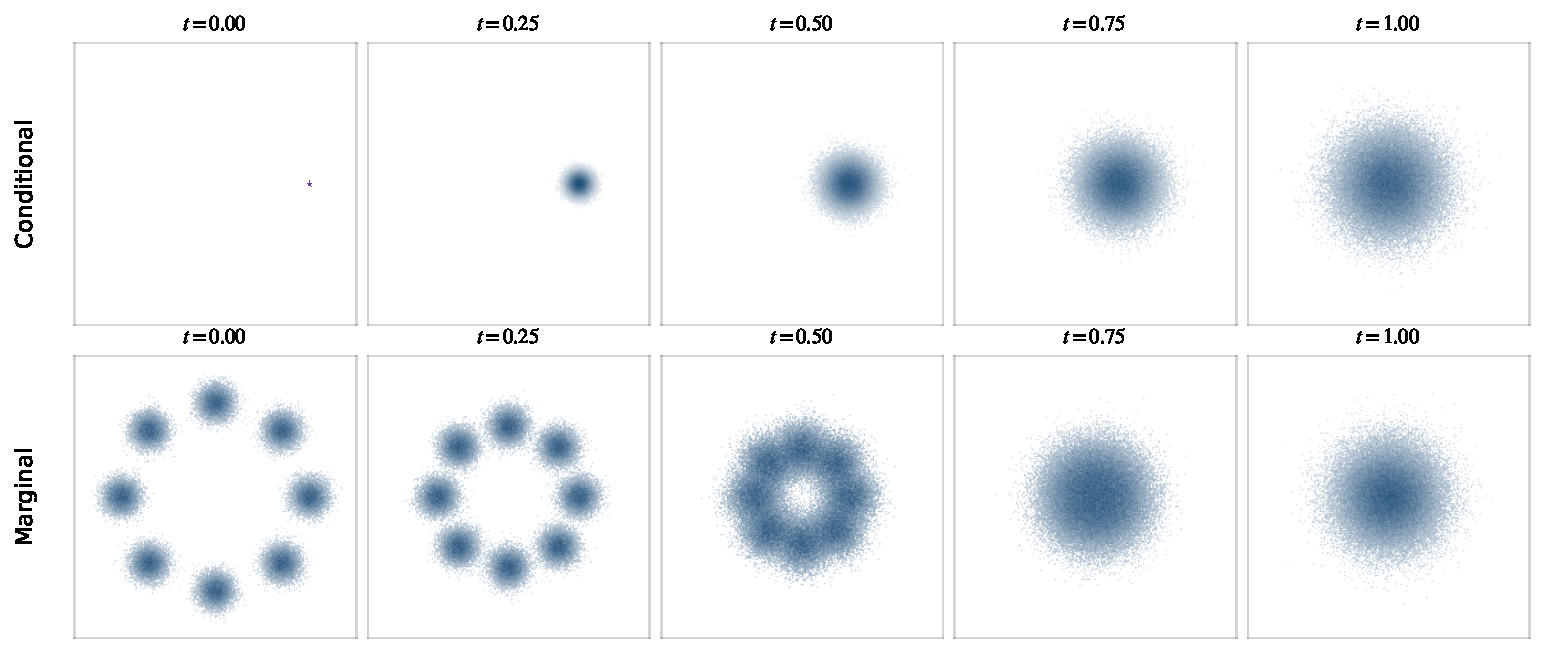
\includegraphics[width=\textwidth]{figures/main_notes/diffusion_models/fig_diffusion_conditional_vs_marginal.pdf}
  \caption{The Gaussian conditional path \eqref{eq:gaussian-conditional-path} for a fixed \(x_0\) (top row) and the induced marginal law \(p_t\) when \(X_0\sim p_0\) (bottom row), illustrated here for the simple choice \(\alpha(t)=1-t\) and \(\sigma(t)=t\).
  Sampling starts from \(p_1\) at \(t=1\) and runs the reverse-time dynamics back to \(t=0\).}
  \label{fig:diffusion-cond-vs-marg}
\end{figure}

The probability path induces a posterior distribution at every time: conditioning on \(X_t=x\) produces a conditional law for the retained endpoint variables, and, if we use a construction like \eqref{eq:stochastic-interpolant-bridge}, for the auxiliary latent variables as well.
This posterior is the exact object from which the reverse kernel is obtained, by the averaging identity above.
In the Euclidean setting we typically do not try to model the full posterior on all latent variables directly.
Instead, the deterministic and stochastic dynamics below depend only on conditional expectations under this posterior, and those expectations are exactly the infinitesimal quantities needed to generate the marginal path.

\subsubsection{Velocity, Endpoint Means, and Score Recovery}

For reverse-time simulation we need a field that depends only on the current state \(x\), not on the hidden variables used to generate the bridge.
The Euclidean tractability move is therefore to replace the full posterior law \(q_{0\mid t}(\cdot\mid x)\) by conditional expectations under it.
For a differentiable interpolant, define the time derivative
\[
  \dot X_t \coloneqq \partial_t I(t,X_0,X_1) + \gamma'(t)\xi,
\]
which still depends on the latent variables and so cannot be used directly as a state-dependent drift.
Its posterior mean is the \emph{velocity field}
\begin{equation}
  b(t,x) \coloneqq \E[\dot X_t \mid X_t=x].
  \label{eq:si-velocity-def}
\end{equation}
This is the primary posterior summary in the continuous-time theory.
See \citet[\S4.1, eqs.~(38)--(40)]{holderrieth_erives_2026_intro_flow_matching} for the same velocity/score/endpoint-mean conversion pattern in a general bridge exposition.
For the linear Gaussian bridge \eqref{eq:gaussian-bridge-path}, it is also useful to introduce the posterior mean of the endpoint at time \(0\),
\begin{equation}
  m(t,x) \coloneqq \E[X_0\mid X_t=x].
  \label{eq:si-endpoint-mean-x0-def}
\end{equation}
Once these two summaries are in hand, the score will follow algebraically from the same Gaussian identities.
For the linear Gaussian bridge \eqref{eq:gaussian-bridge-path}, we have
\[
  \dot X_t = \alpha'(t)X_0 + \sigma'(t)Z,
\]
so \(b(t,x)=\E[\alpha'(t)X_0+\sigma'(t)Z\mid X_t=x]\).
Moreover, conditioning on \((X_0,X_t)=(x_0,x)\) yields
\[
  \E[\dot X_t\mid X_0=x_0,X_t=x]
  =
  \alpha'(t)x_0
  +
  \frac{\sigma'(t)}{\sigma(t)}\bigl(x-\alpha(t)x_0\bigr),
\]
which is the closed-form conditional vector field used in conditional flow matching.
The score field \(s(t,x)\coloneqq \nabla\log p_t(x)\) is then determined by \(b\) as well.

\begin{proposition}[Derived endpoint mean and score for the linear Gaussian bridge]
\label{prop:score-from-endpoint-mean}
Assume \eqref{eq:gaussian-bridge-path} holds with smooth functions \(\alpha,\sigma\) such that \(\sigma(t)>0\) and
\[
  D(t)\coloneqq \alpha(t)\sigma'(t)-\sigma(t)\alpha'(t)\neq 0
\]
for \(t\in(0,1]\).
Fix \(t\in(0,1]\).
Assume \(x\mapsto K_{t\mid 0}(x\mid x_0)\) is \(C^1\) for every \(x_0\), that differentiation with respect to \(x\) may be passed through the mixture formula \eqref{eq:marginal-mixture-path}, and that \(p_t(x)>0\) at the points where the score identity is evaluated.
Then:
\begin{enumerate}[leftmargin=*]
  \item The endpoint posterior mean is determined by the velocity:
  \begin{equation}
    m(t,x) = \frac{\sigma'(t)x-\sigma(t)b(t,x)}{D(t)}.
    \label{eq:endpoint-mean-from-velocity}
  \end{equation}
  \item The score can be written in terms of the endpoint mean (equivalently, in terms of \(b\)):
  \begin{equation}
    \nabla\log p_t(x)
    =
    -\frac{1}{\sigma(t)^2}\Bigl(x-\alpha(t)\,m(t,x)\Bigr)
    =
    \frac{\alpha'(t)x-\alpha(t)b(t,x)}{\sigma(t)D(t)}.
    \label{eq:score-from-endpoint-mean}
  \end{equation}
\end{enumerate}
\end{proposition}
\begin{proof}
Define
\[
  n(t,x)\coloneqq \E[Z\mid X_t=x].
\]
Taking conditional expectations in \eqref{eq:gaussian-bridge-path} gives
\[
  x = \alpha(t)\E[X_0\mid X_t=x] + \sigma(t)\E[Z\mid X_t=x]
  = \alpha(t)m(t,x)+\sigma(t)n(t,x).
\]
Likewise,
\[
  b(t,x)=\alpha'(t)m(t,x)+\sigma'(t)n(t,x).
\]
Eliminating \(n(t,x)\) from these two equations yields
\[
  D(t)m(t,x)=\sigma'(t)x-\sigma(t)b(t,x),
\]
which proves \eqref{eq:endpoint-mean-from-velocity}.

For the score, conditioned on \(X_0\), \eqref{eq:gaussian-conditional-path} gives the density
\[
  K_{t\mid 0}(x\mid X_0)
  \propto
  \exp\!\left(-\frac{1}{2\sigma(t)^2}\norm{x-\alpha(t)X_0}_2^2\right).
\]
Differentiating with respect to \(x\) yields
\[
  \nabla_x\log K_{t\mid 0}(x\mid X_0)
  =
  -\frac{x-\alpha(t)X_0}{\sigma(t)^2}.
\]
By \eqref{eq:marginal-mixture-path} and differentiation under the integral sign,
\[
  \nabla p_t(x)
  =
  \int_{\R^d}\nabla_x K_{t\mid 0}(x\mid x_0)\,p_0(x_0)\,dx_0.
\]
Since \(p_t(x)>0\), we may divide by \(p_t(x)\) and use \(\nabla_x K_{t\mid 0}=K_{t\mid 0}\nabla_x\log K_{t\mid 0}\) to obtain
\begin{align*}
  \nabla\log p_t(x)
  &=
  \frac{1}{p_t(x)}
  \int_{\R^d}\nabla_x K_{t\mid 0}(x\mid x_0)\,p_0(x_0)\,dx_0 \\
  &=
  \int_{\R^d}\nabla_x\log K_{t\mid 0}(x\mid x_0)\,
  \frac{K_{t\mid 0}(x\mid x_0)\,p_0(x_0)}{p_t(x)}\,dx_0.
\end{align*}
The factor multiplying \(\nabla_x\log K_{t\mid 0}\) is exactly the posterior density of \(X_0\) given \(X_t=x\), so this is the Fisher-type identity
\[
  \nabla\log p_t(x)
  =
  \E\!\left[\nabla_x\log K_{t\mid 0}(x\mid X_0)\mid X_t=x\right].
\]
Substituting the Gaussian score from above gives
\[
  \nabla\log p_t(x)
  =
  -\frac{1}{\sigma(t)^2}\,\E\!\left[x-\alpha(t)X_0\mid X_t=x\right]
  =
  -\frac{1}{\sigma(t)^2}\Bigl(x-\alpha(t)m(t,x)\Bigr),
\]
which is the first identity in \eqref{eq:score-from-endpoint-mean}.
Using \(x-\alpha(t)m(t,x)=\sigma(t)n(t,x)\) and eliminating \(m(t,x)\) instead gives
\[
  D(t)n(t,x)=\alpha(t)b(t,x)-\alpha'(t)x,
\]
hence
\[
  \nabla\log p_t(x)
  =
  -\frac{n(t,x)}{\sigma(t)}
  =
  \frac{\alpha'(t)x-\alpha(t)b(t,x)}{\sigma(t)D(t)}.
\]
This is the second identity in \eqref{eq:score-from-endpoint-mean}.
\end{proof}

The practical lesson is that the Gaussian bridge turns the full posterior law into a small menu of interchangeable posterior summaries.
One may learn the velocity field, the endpoint posterior mean, the Gaussian innovation predictor, or the score.
For this bridge these are not different conceptual objects; they are linear reparameterizations of the same posterior information.

\subsubsection{Density evolution and common-marginal dynamics}
\label{subsubsec:diffusion-density-evolution}

The velocity field \(b\) transports the marginal density \(p_t\).
One realization of this path is the deterministic probability-flow ODE with drift \(b\), and in flow matching this is the core marginalization trick: one can define a marginal vector field by averaging simple conditional velocities under the posterior, and this marginal vector field exactly generates the marginal probability path \citep[\S3.1]{lipman_chen_ben_hamu_nickel_le_2023_flow_matching}; see also \citet[Thm.~11]{holderrieth_erives_2026_intro_flow_matching}.

\begin{proposition}[Transport equation for the bridge marginals]
\label{prop:si-transport-equation}
Assume \(t\mapsto X_t\) is differentiable almost surely and that \(X_t\) has a density \(p_t\) for every \(t\in[0,1]\).
Let \(b\) be defined by \eqref{eq:si-velocity-def}.
Then \(p_t\) satisfies
\begin{equation}
  \partial_t p_t(x) + \nabla\cdot\bigl(b(t,x)p_t(x)\bigr)=0.
  \label{eq:si-transport-equation}
\end{equation}
\end{proposition}
\begin{proof}
Let \(\varphi\in C_0^\infty(\R^d)\).
Differentiate \(\varphi(X_t)\) using \(\dot X_t\) and take expectations:
\[
  \frac{d}{dt}\E[\varphi(X_t)]
  =
  \E\!\left[\ip{\nabla\varphi(X_t)}{\dot X_t}\right]
  =
  \E\!\left[\ip{\nabla\varphi(X_t)}{\E[\dot X_t\mid X_t]}\right]
  =
  \int_{\R^d}\ip{\nabla\varphi(x)}{b(t,x)}p_t(x)\,dx.
\]
Integrating by parts yields the weak form of \eqref{eq:si-transport-equation}.
\end{proof}

Once \(p_t\) and \(b\) are fixed, there is no reason to privilege a single trajectory-level dynamics.
The same forward law can be realized by a whole family of reverse-time diffusions and ODEs.
For sampling, the stochastic realizations are especially natural, while the probability-flow ODE appears as the zero-noise member of the same family.
This common-marginal viewpoint is formalized by \citet[\S2]{albergo_boffi_vanden_eijnden_2025_stochastic_interpolants} and \citet[Thm.~17]{holderrieth_erives_2026_intro_flow_matching}.

\begin{proposition}[A common-marginal family of dynamics]
\label{prop:si-family-of-sdes}
Assume that for each \(t\in(0,1)\), the density \(p_t\) is \(C^2\) and strictly positive on \(\R^d\).
Let \(s(t,x)\coloneqq\nabla\log p_t(x)\), and assume the Fokker--Planck equations below are well posed for the initial data considered.
Fix any continuous schedule \(\varepsilon:[0,1]\to[0,\infty)\) and define
\begin{equation}
  b_{\mathrm{fwd}}(t,x) \coloneqq b(t,x) + \varepsilon(t)s(t,x),
  \qquad
  b_{\mathrm{rev}}(t,x) \coloneqq b(t,x) - \varepsilon(t)s(t,x).
  \label{eq:si-forward-backward-drifts}
\end{equation}
Consider the forward and reverse-time dynamics
\begin{equation}
  dY_t^{\mathrm{fwd}}=b_{\mathrm{fwd}}(t,Y_t^{\mathrm{fwd}})\,dt+\sqrt{2\,\varepsilon(t)}\,dB_t,
  \qquad
  dY_t^{\mathrm{rev}}=b_{\mathrm{rev}}(t,Y_t^{\mathrm{rev}})\,dt+\sqrt{2\,\varepsilon(t)}\,dB_t,
  \label{eq:si-forward-backward-sdes}
\end{equation}
where the second equation is simulated backward in time from \(t=1\) to \(t=0\).
When \(\varepsilon\equiv 0\), these reduce to deterministic ODEs with drift \(b\).
Then:
\begin{enumerate}[leftmargin=*]
  \item If \(Y_0^{\mathrm{fwd}}\sim p_0\), then the time-marginal density of \((Y_t^{\mathrm{fwd}})\) is \(p_t\) for every \(t\in[0,1]\).
  \item If \(Y_1^{\mathrm{rev}}\sim p_1\), then the reverse-time marginal density of \((Y_t^{\mathrm{rev}})\) at time \(t\) is also \(p_t\).
\end{enumerate}
\end{proposition}
\begin{proof}
If \(\varepsilon\equiv 0\), then the first claim is exactly the transport equation \eqref{eq:si-transport-equation} written in trajectory form.
Assume now that \(\varepsilon\) is arbitrary.
The density \(\rho\) of \((Y_t^{\mathrm{fwd}})\) then satisfies the forward Fokker--Planck equation
\[
  \partial_t \rho + \nabla\cdot\bigl((b+\varepsilon s)\rho\bigr) = \varepsilon \Delta\rho.
\]
To identify the solution, observe that \(p_t\) itself satisfies the same PDE:
\[
  \partial_t p_t + \nabla\cdot\bigl((b+\varepsilon s)p_t\bigr)
  =
  \partial_t p_t + \nabla\cdot(bp_t) + \varepsilon\nabla\cdot(sp_t).
\]
By \eqref{eq:si-transport-equation}, the first two terms sum to zero, while
\[
  \nabla\cdot(sp_t)
  =
  \nabla\cdot\bigl((\nabla\log p_t)p_t\bigr)
  =
  \nabla\cdot(\nabla p_t)
  =
  \Delta p_t.
\]
Hence \(p_t\) solves the forward Fokker--Planck equation with initial condition \(p_0\).
By well posedness, \(\rho_t=p_t\) for all \(t\in[0,1]\).

For the second claim, set \(\tau\coloneqq 1-t\) and define \(\bar p_\tau(x)\coloneqq p_{1-\tau}(x)\).
Then
\[
  \partial_\tau \bar p_\tau(x)
  =
  -\partial_t p_t(x)\vert_{t=1-\tau}
  =
  \nabla\cdot\bigl(b(1-\tau,x)\bar p_\tau(x)\bigr)
\]
by \eqref{eq:si-transport-equation}.
Now consider the forward-in-\(\tau\) process associated with backward simulation in \(t\):
\[
  d\bar Y_\tau
  =
  -b_{\mathrm{rev}}(1-\tau,\bar Y_\tau)\,d\tau
  +
  \sqrt{2\,\varepsilon(1-\tau)}\,d\bar B_\tau.
\]
Its density \(\bar \rho_\tau\) satisfies
\[
  \partial_\tau \bar \rho_\tau
  +
  \nabla\cdot\bigl(-b_{\mathrm{rev}}(1-\tau,\cdot)\bar \rho_\tau\bigr)
  =
  \varepsilon(1-\tau)\Delta\bar \rho_\tau.
\]
Using \(b_{\mathrm{rev}}=b-\varepsilon s\), the candidate path \(\bar p_\tau\) obeys
\[
  \partial_\tau \bar p_\tau
  +
  \nabla\cdot\bigl((-b+\varepsilon s)(1-\tau,\cdot)\bar p_\tau\bigr)
  =
  \varepsilon(1-\tau)\nabla\cdot\bigl(s(1-\tau,\cdot)\bar p_\tau\bigr)
  =
  \varepsilon(1-\tau)\Delta\bar p_\tau.
\]
Thus \(\bar p_\tau\) solves the forward Fokker--Planck equation for the time-reversed simulation, with initial condition \(\bar p_0=p_1\).
By well posedness, \(\bar \rho_\tau=\bar p_\tau\).
Translating back to the original time variable \(t\) yields the stated reverse-time simulation property.
\end{proof}

\begin{corollary}[Langevin as a stationary-path special case]
\label{cor:langevin-stationary-path}
Suppose \(p_t\equiv \pi\) is constant in time, \(b\equiv 0\), and \(\varepsilon(t)\equiv 1\).
Then the forward member of \eqref{eq:si-forward-backward-sdes} is
\[
  dY_t = \nabla\log \pi(Y_t)\,dt + \sqrt{2}\,dB_t,
\]
which is exactly the overdamped Langevin diffusion from \Cref{subsubsec:langevin-diffusion}, and every marginal law is \(\pi\).
\end{corollary}
This is the course-level payoff of the common-marginal viewpoint.
The same drift-noise template governs stationary MCMC and time-inhomogeneous diffusion samplers; what changes is whether the target law is fixed or moves along the bridge.

\begin{figure}[t]
  \centering
  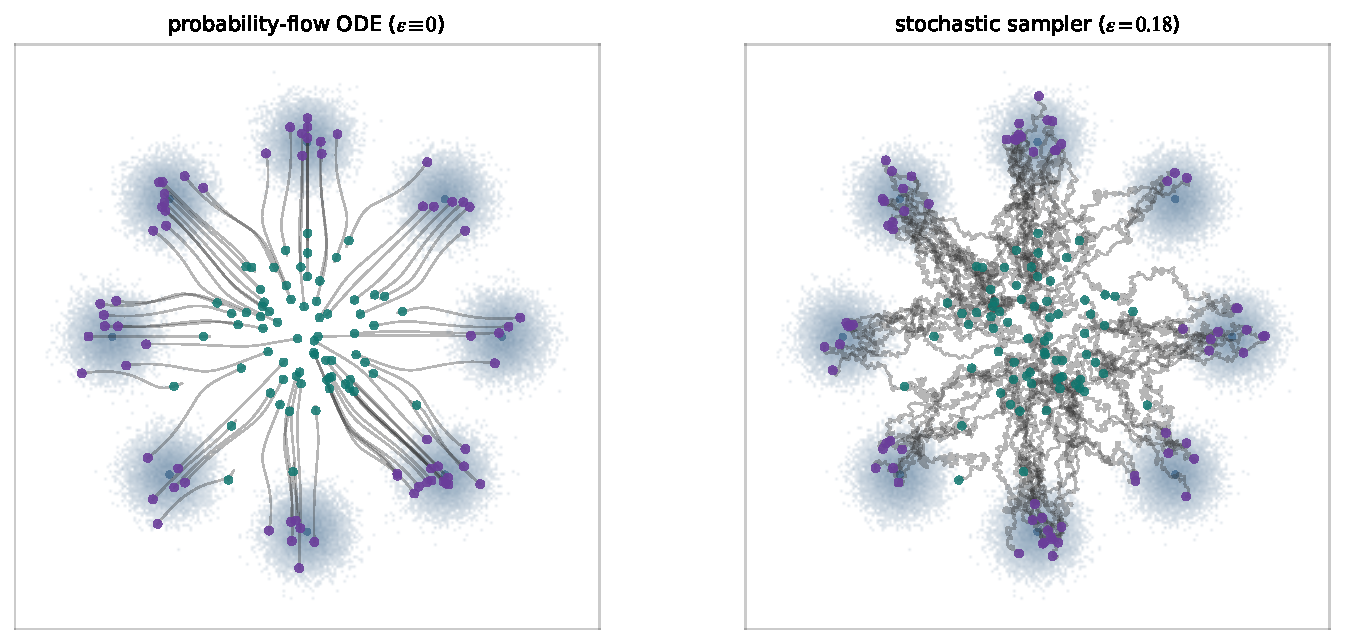
\includegraphics[width=\textwidth]{figures/main_notes/diffusion_models/fig_diffusion_reverse_dynamics.pdf}
  \caption{Reverse-time simulation from \(p_1\) back to \(p_0\) for a toy two-dimensional data distribution.
  Different choices of the noise schedule \(\varepsilon\) in \eqref{eq:si-forward-backward-sdes} produce different sample trajectories while preserving the same marginal path \(p_t\).
  The probability-flow ODE is the zero-noise case \(\varepsilon\equiv 0\).}
  \label{fig:diffusion-reverse-dynamics}
\end{figure}
